\documentclass[11pt,a4paper]{article}
\usepackage[margin=2.3cm]{geometry}
\usepackage{amsmath,amssymb,booktabs,graphicx,braket}
\usepackage[font=small,labelfont=bf]{caption}
\usepackage[hidelinks]{hyperref}
\graphicspath{{../results/}}
\setlength{\parskip}{0.45em}
\setlength{\parindent}{0pt}

\title{\textbf{How long can a matrix product state follow a mirror circuit?}\\[0.3em]
\large A small simulation study of the simplest peaked circuits}
\author{Pham Quang Minh\\
\small Ho Chi Minh City University of Technology (HCMUT)\\
\small Code: \url{https://github.com/USERNAME/REPO}}
\date{November 2026}

\begin{document}
\maketitle

\begin{abstract}
\noindent Peaked circuits are quantum circuits that look random but output one bitstring with
high probability. They have been proposed as a test of quantum advantage that is easy to
verify. In this report I study the simplest example, a mirror circuit, with a matrix product
state (MPS) simulator that I wrote in NumPy. The simulator applies the gates in order and
truncates each bond to a fixed dimension $\chi$. On 16 qubits, the probability that the
simulator gives to the correct bitstring falls smoothly with depth and follows the
entanglement entropy at the middle of the circuit. With $\chi=64$ it is still $0.46$ after
480 two-qubit gates, which is about $3\times10^{4}$ times a random guess, so the answer can
still be read off by sampling. A 48-qubit circuit of half-depth 8 takes about one second.
I also include a short second experiment comparing amplitude estimation with Monte Carlo
sampling. The main limitation is that mirror circuits are much easier than the peaked
circuits used in the literature.
\end{abstract}

\section{Introduction}

A quantum computer with $n$ qubits has a state with $2^n$ amplitudes, so simulating it
exactly on a classical computer becomes impossible at around 45 to 50 qubits. Experiments
that claim quantum advantage rely on this. The problem is checking the answer: if no
classical computer can simulate the circuit, it is hard to know that the quantum computer
was right.

Peaked circuits were proposed by Aaronson and Zhang \cite{aaronson2024} to deal with this.
A peaked circuit looks like a random circuit, but its output distribution has one bitstring
with unusually high probability. The quantum computer finds this bitstring by running the
circuit and measuring a few times, and anyone can check it. The test only works if classical
simulators cannot find the same bitstring. A later paper ran peaked circuits with about
2000 two-qubit gates on a trapped-ion device and compared against tensor-network and
Pauli-path simulators \cite{gharibyan2025}.

I arrived at this question from a different direction. My first experiment
(Section~\ref{sec:ae}) simulated quantum amplitude estimation for a counting task from my
recommender-system capstone. It beat random sampling by a factor of 17 at equal queries, but
when the data was sorted, the quantum state could be stored as a tensor network of only 104
numbers, so a classical computer could reproduce it easily. Whether there was an advantage
depended on the structure of the problem. That made me want to understand the classical side
in the smallest setting I could build myself. My question is:

\begin{quote}
For the simplest peaked circuits, how does the bond dimension of an MPS simulator limit its
ability to find the peak as the circuit gets deeper?
\end{quote}

I use mirror circuits (a random circuit followed by its inverse), which are a standard tool
in benchmarking \cite{proctor2022}. They are peaked by construction. They are also easy in a
way real peaked circuits are not, and I come back to this in Section~\ref{sec:limits}.

\section{Background}

\subsection{Matrix product states}

An MPS writes the $2^n$ amplitudes of a state as a product of $n$ small tensors,
\begin{equation}
\psi_{b_1 b_2 \dots b_n} = A^{[1]}_{b_1} A^{[2]}_{b_2} \cdots A^{[n]}_{b_n},
\end{equation}
where each $A^{[i]}_{b_i}$ is a matrix of size at most $\chi\times\chi$ and $b_i\in\{0,1\}$
\cite{vidal2003,schollwock2011}. The number $\chi$ is the bond dimension. Storage is
$O(n\chi^2)$ numbers and not $2^n$.

The price is that an MPS with bond dimension $\chi$ can hold at most $\log_2\chi$ bits of
entanglement entropy across any cut of the chain. A product state has $\chi=1$ and a GHZ
state has $\chi=2$. A typical random state on $n$ qubits needs $\chi=2^{n/2}$.

To apply a two-qubit gate on neighbouring sites $i$ and $i+1$, the two tensors are
contracted, the gate is applied, and the result is split again with a singular value
decomposition (SVD). If there are more than $\chi$ singular values, only the largest $\chi$
are kept. This is where the error comes from. Each SVD costs $O(\chi^3)$.

\subsection{Mirror circuits}

Let $U$ be a circuit of $d$ layers of random two-qubit gates. The mirror circuit is
\begin{equation}
C = X^{s}\, U^{\dagger} U ,
\end{equation}
where $X^{s}$ applies an $X$ gate to every qubit $i$ with $s_i=1$, for a random bitstring
$s$. Since $U^\dagger U = I$, the output is exactly $\ket{s}$. I call $d$ the half-depth.
The entanglement is largest in the middle, after $U$, and returns to zero at the end.

\section{Method}

\textbf{Circuits.} $U$ is a brickwork circuit on a line of $n$ qubits. Layer $\ell$ puts a
Haar-random two-qubit gate on bonds $(i,i+1)$ with $i\equiv\ell \pmod 2$. A circuit with
$n=16$ and $d=32$ has 480 two-qubit gates.

\textbf{Simulator.} I wrote the MPS simulator in NumPy (file \texttt{peaked.py}, about 100
lines). It keeps the MPS in canonical form by moving the orthogonality centre with QR
decompositions before each gate, so that the SVD truncation is the optimal one for that
bond. After truncation the singular values are renormalised. The simulator is given the
gates of $C$ as a flat list. It does not know that the second half is the inverse of the
first.

\textbf{What I measure.} The main quantity is $p_\chi(s)=|\braket{s|\psi_\chi}|^2$, the
probability that the truncated MPS gives to the correct bitstring. Without truncation it is
1. For comparison, a random guess has probability $2^{-n}$. I also compute the
entanglement entropy across the middle cut after the forward half $U$,
$S=-\sum_k \lambda_k^2 \log_2 \lambda_k^2$, from an exact state-vector simulation, where
$\lambda_k$ are the Schmidt coefficients.

\textbf{Checks.} The tests compare the MPS with an exact state vector on 8 qubits (agreement
to $10^{-10}$ when $\chi$ is not limiting), check that the mirror circuit output has
probability 1 on $s$, and check that a GHZ state is represented exactly with $\chi=2$.

\textbf{Setup.} All runs use one core of an Apple M4 laptop with 16 GB of memory. Each data
point for $n=16$ is the mean over 5 random circuits. Everything can be reproduced with
\texttt{python run\_peaked.py} (about 35 seconds).

\section{Results}

\subsection{Peak probability against depth and bond dimension}

\begin{figure}[h]
\centering
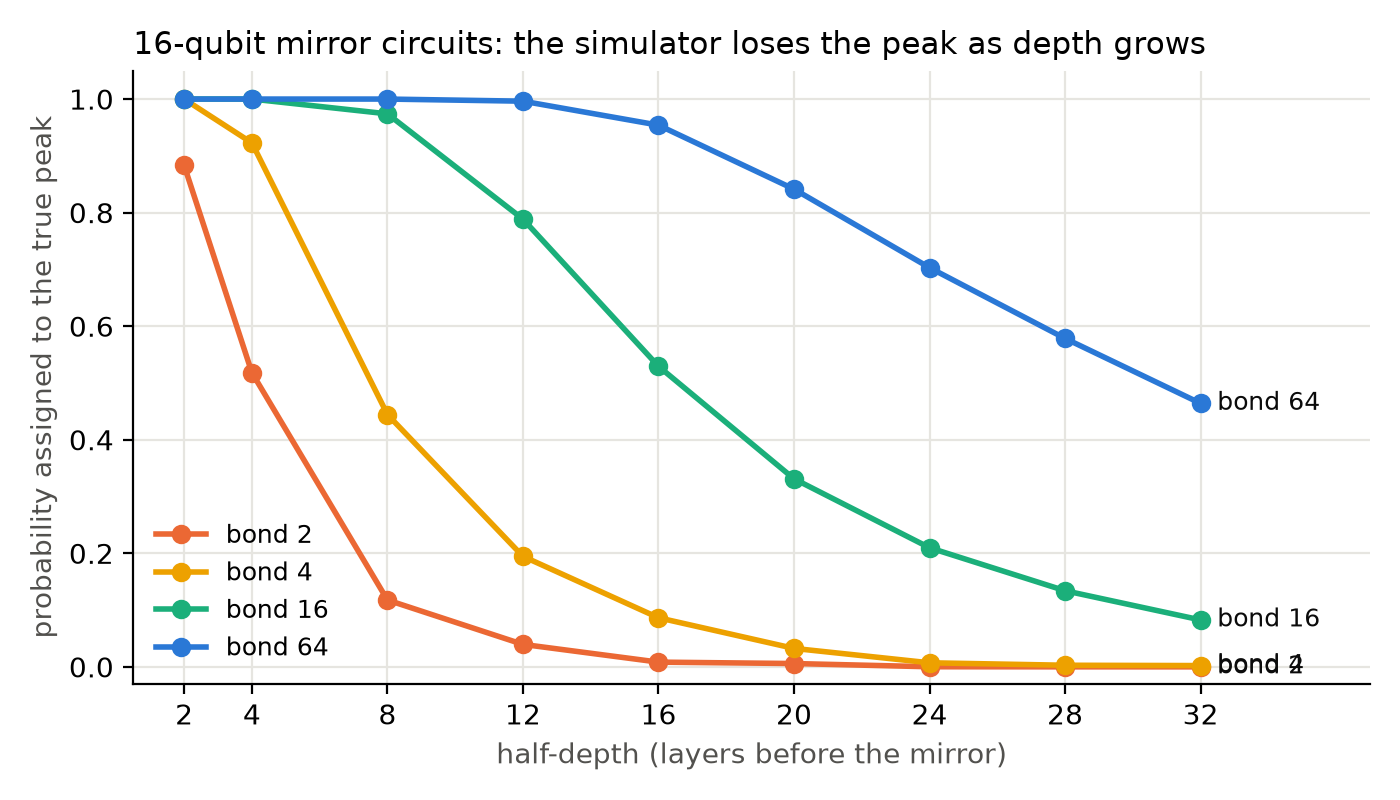
\includegraphics[width=0.78\linewidth]{fig_peak_recovery.png}
\caption{Probability given to the correct bitstring by the truncated MPS, for 16-qubit
mirror circuits. Mean over 5 circuits per point.}
\label{fig:recovery}
\end{figure}

\begin{table}[h]
\centering\small
\begin{tabular}{@{}rrrcccc@{}}
\toprule
$d$ & gates & $S$ (bits) & $\chi=2$ & $\chi=4$ & $\chi=16$ & $\chi=64$ \\
\midrule
2 & 30 & 0.76 & 0.883 & 1.000 & 1.000 & 1.000 \\
4 & 60 & 1.68 & 0.518 & 0.923 & 1.000 & 1.000 \\
8 & 120 & 3.20 & 0.118 & 0.444 & 0.974 & 1.000 \\
12 & 180 & 4.47 & 0.040 & 0.195 & 0.789 & 0.996 \\
16 & 240 & 5.64 & 0.008 & 0.086 & 0.529 & 0.954 \\
20 & 300 & 6.49 & 0.006 & 0.032 & 0.331 & 0.841 \\
24 & 360 & 6.95 & 0.000 & 0.007 & 0.210 & 0.703 \\
28 & 420 & 7.13 & 0.000 & 0.003 & 0.134 & 0.578 \\
32 & 480 & 7.22 & 0.000 & 0.002 & 0.083 & 0.464 \\
\bottomrule
\end{tabular}
\caption{$p_\chi(s)$ for $n=16$. $d$ is the half-depth and $S$ is the entropy across the
middle cut after the forward half (maximum 8 bits).}
\label{tab:recovery}
\end{table}

Figure~\ref{fig:recovery} and Table~\ref{tab:recovery} show three things.

First, the peak probability falls smoothly. There is no sharp depth at which the simulator
stops working.

Second, the fall follows the entropy $S$. A bond dimension $\chi$ can hold $\log_2\chi$
bits. For $\chi=4$ (2 bits) the probability is still 0.92 at $S=1.68$ and has dropped to
0.44 at $S=3.20$. For $\chi=16$ (4 bits) it is 0.97 at $S=3.20$ and 0.79 at $S=4.47$. For
$\chi=64$ (6 bits) it is 0.95 at $S=5.64$ and 0.84 at $S=6.49$. In each case the simulator
starts to lose the peak when $S$ gets close to $\log_2\chi$.

Third, the simulator can find the peak even when it represents the state badly. At $d=32$
with $\chi=64$ the peak probability is 0.46, and with $\chi=16$ it is 0.083. A random guess
is $2^{-16}\approx1.5\times10^{-5}$. So with $\chi=16$ the correct string is still about
5000 times more likely than a random one and would show up after a few dozen samples. Only
$\chi=2$ and $\chi=4$ really lose the answer at large depth.

The entropy grows slowly in these circuits. It rises by about 0.4 bits per layer for the
first 8 layers and then levels off near 7.2 bits, slightly under the maximum of 8.

\subsection{Run time}

\begin{figure}[h]
\centering
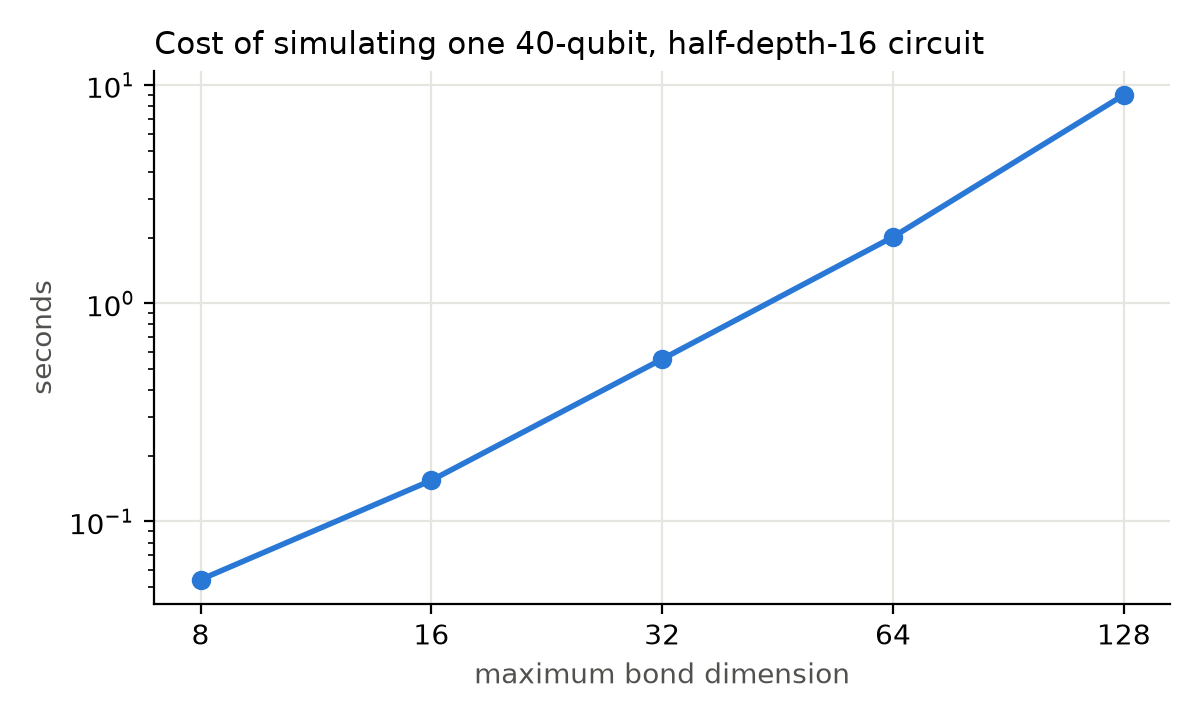
\includegraphics[width=0.55\linewidth]{fig_peak_cost.png}
\caption{Run time against bond dimension for one circuit with 40 qubits and half-depth 16
(639 gates).}
\label{fig:cost}
\end{figure}

For a 40-qubit circuit with 639 gates, the run time grows from 0.05 s at $\chi=8$ to 9.0 s at
$\chi=128$ (Figure~\ref{fig:cost}). A fit to the last three points gives an exponent of about
2.0. The SVD cost should give $\chi^3$ for large $\chi$. I think the matrices here (at most
$256\times256$) are small enough that overheads other than the SVD still matter, but I did
not profile it.

\subsection{A case that a state vector cannot hold}

I ran one 48-qubit mirror circuit with half-depth 8 and $\chi=64$. The simulation took
1.05 s and the MPS used 4.9 MB. The correct bitstring got probability 0.9999, and a single
sample from the MPS returned it. A state vector for 48 qubits would need about 4500 TB. This
case is easy for the MPS because at half-depth 8 the entropy is only about 3 bits. There is
no exact result to compare with at this size, but for a mirror circuit the correct answer is
known by construction.

\section{Where the question came from: amplitude estimation}
\label{sec:ae}

This was my first experiment, and it is related to my capstone on recommender systems. Given a catalogue of $N$ items where a fraction $a$ are relevant to a
user, how many queries are needed to estimate $a$?

Classical Monte Carlo sampling has error proportional to $1/\sqrt{M}$ for $M$ queries.
Quantum amplitude estimation \cite{brassard2002} has error proportional to $1/M$. I used the
maximum likelihood version \cite{suzuki2020}, which runs Grover circuits with $k$ iterations
for several values of $k$ and uses the fact that the probability of measuring a relevant
item is $\sin^2((2k+1)\theta)$ with $a=\sin^2\theta$. I also limited $k$ to a maximum
depth, because deep circuits are hard to run on real devices \cite{vu2024}.

\begin{figure}[h]
\centering
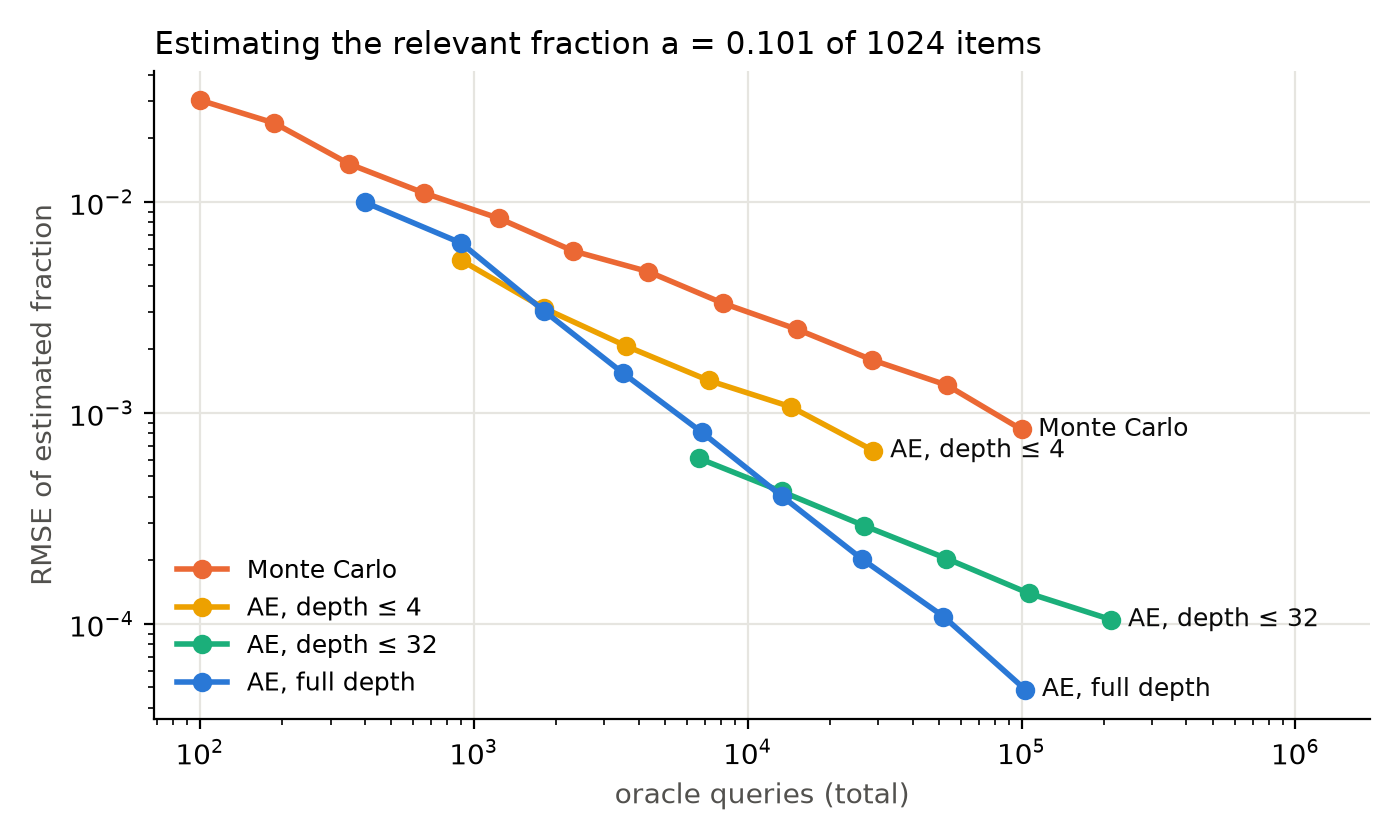
\includegraphics[width=0.7\linewidth]{fig_accuracy.png}
\caption{Error against total number of oracle queries, for $N=1024$ and $a=0.10$. RMSE over
200 trials.}
\label{fig:ae}
\end{figure}

\begin{table}[h]
\centering\small
\begin{tabular}{@{}lcc@{}}
\toprule
Method & fitted exponent & RMSE near $10^5$ queries \\
\midrule
Monte Carlo & $-0.50$ & $8.3\times10^{-4}$ \\
Amplitude estimation, $k\le32$ & $-0.51$ & $1.4\times10^{-4}$ \\
Amplitude estimation, full depth ($k\le256$) & $-0.98$ & $4.9\times10^{-5}$ \\
\bottomrule
\end{tabular}
\caption{Amplitude estimation against Monte Carlo.}
\label{tab:ae}
\end{table}

Full-depth amplitude estimation was about 17 times more accurate than Monte Carlo at the
same number of queries (Table~\ref{tab:ae}). Limiting the depth to 32 kept a factor of about
6, but the exponent went back to $-0.5$. These numbers agree with what is already known, so
this part is a check of my understanding and not a new result.

The last observation is the one that led to the rest of this report. I converted the Grover state for 14 qubits to an
MPS. When the relevant items are at random positions in the catalogue, the state needs
$\chi=128$, the maximum. When the catalogue is sorted so the relevant items form one block,
it needs only $\chi=2$. So whether this problem is hard to simulate depends on how the data
is arranged.

\section{Discussion and limitations}
\label{sec:limits}

The main result is that for 1D mirror circuits a truncated MPS keeps finding the peak well
after its fidelity with the true state has become small. This is good for the simulator and
means that these circuits would be a poor test of quantum advantage. Zhou, Stoudenmire and
Waintal \cite{zhou2020} studied how the fidelity of truncated MPS simulations decays with
the number of gates for random circuits. My results are consistent with a gradual decay, but
I measure a different quantity (the probability of one bitstring), and I have not compared
the two carefully.

There are several limitations.

\textbf{Mirror circuits are the easy case.} The structure $U^\dagger U$ is visible in the
gate list, so a simulator could simply cancel the gates. My simulator does not do this, but
the circuits are still much weaker than those of \cite{aaronson2024,gharibyan2025}, where
the peak is produced by trained or hidden layers and cannot be removed by inspection.

\textbf{One dimension.} All gates act on neighbours on a line. Entanglement grows faster
with 2D or all-to-all connectivity, which is what the trapped-ion experiments use. An MPS is
expected to do much worse there.

\textbf{Small sizes and few samples.} The main table uses 16 qubits and 5 circuits per
point, and I do not report error bars. The run-time fit uses three points.

\textbf{One method.} I only tested an MPS. The literature also uses tensor networks with
belief propagation and Pauli-path methods \cite{gharibyan2025}.

\textbf{No noise.} All simulations are noiseless.

\section{Future work}

\begin{enumerate}
\setlength{\itemsep}{0pt}
\item Implement the construction of \cite{aaronson2024} for 8 to 12 qubits, where the
second half of the circuit is trained to produce a peak, and repeat the experiment.
\item Check the simulator against an established library such as quimb.
\item Replace the 1D layout with a 2D grid and with all-to-all gates, and measure how the
required bond dimension changes.
\item Move the SVDs to a GPU and see at what bond dimension that starts to help.
\end{enumerate}

\begin{thebibliography}{9}\small
\setlength{\itemsep}{0pt}
\bibitem{aaronson2024} S.~Aaronson and Y.~Zhang. On verifiable quantum advantage with peaked
circuit sampling. arXiv:2404.14493, 2024.
\bibitem{gharibyan2025} H.~Gharibyan, M.~Z.~Mullath, N.~E.~Sherman, V.~P.~Su, H.~Tepanyan
and Y.~Zhang. Heuristic quantum advantage with peaked circuits. arXiv:2510.25838, 2025.
\bibitem{proctor2022} T.~Proctor, K.~Rudinger, K.~Young, E.~Nielsen and R.~Blume-Kohout.
Measuring the capabilities of quantum computers. \emph{Nature Physics} 18, 75--79, 2022.
\bibitem{vidal2003} G.~Vidal. Efficient classical simulation of slightly entangled quantum
computations. \emph{Physical Review Letters} 91, 147902, 2003.
\bibitem{schollwock2011} U.~Schollw\"ock. The density-matrix renormalization group in the
age of matrix product states. \emph{Annals of Physics} 326, 96--192, 2011.
\bibitem{zhou2020} Y.~Zhou, E.~M.~Stoudenmire and X.~Waintal. What limits the simulation of
quantum computers? \emph{Physical Review X} 10, 041038, 2020.
\bibitem{brassard2002} G.~Brassard, P.~H\o yer, M.~Mosca and A.~Tapp. Quantum amplitude
amplification and estimation. \emph{Contemporary Mathematics} 305, 53--74, 2002.
\bibitem{suzuki2020} Y.~Suzuki, S.~Uno, R.~Raymond, T.~Tanaka, T.~Onodera and N.~Yamamoto.
Amplitude estimation without phase estimation. \emph{Quantum Information Processing} 19, 75,
2020.
\bibitem{vu2024} D.-L.~Vu, B.~Cheng and P.~Rebentrost. Low depth amplitude estimation
without really trying. arXiv:2410.01173, 2024.
\end{thebibliography}

\end{document}
